\documentclass[11pt,a4paper]{article}
\usepackage{fontspec}
\setmainfont{TeX Gyre Pagella}
\newfontfamily\headfont{Inter}[UprightFont=*-ExtraBold,BoldFont=*-ExtraBold,Extension=.otf,Path=/usr/share/fonts/opentype/inter/]
\usepackage[a4paper,margin=2.3cm]{geometry}
\usepackage{graphicx,booktabs,float,caption,array,xcolor}
\usepackage[hidelinks]{hyperref}
\usepackage{titlesec}
\usepackage[round]{natbib}
\usepackage{setspace}
\setstretch{1.05}
\renewcommand{\topfraction}{0.9}
\renewcommand{\bottomfraction}{0.8}
\renewcommand{\textfraction}{0.1}
\renewcommand{\floatpagefraction}{0.75}
\setlength{\parindent}{0pt}
\setlength{\parskip}{0.55em}
\titleformat{\section}{\headfont\Large}{\thesection}{0.8em}{}
\titleformat{\subsection}{\headfont\large}{\thesubsection}{0.8em}{}
\captionsetup{font=small,labelfont=bf}
\urlstyle{same}
\hypersetup{pdftitle={What's Left of the Workhouse? Traces of Britain and Ireland's Workhouses in Open Data},pdfauthor={Tristan Hotham}}

\begin{document}
\begin{center}
{\Large\bfseries What's Left of the Workhouse?\par}
\vspace{0.4em}
{\large Traces of Britain and Ireland's workhouses in listed building registers,\\OpenStreetMap, Wikidata and Wikipedia\par}
\vspace{1.2em}
{\large Tristan Hotham\par}
\vspace{0.3em}
{\small Independent researcher\\
ORCID: 0000-0003-4931-9349\\
DOI: \href{https://doi.org/10.5281/zenodo.23844517}{https://doi.org/10.5281/zenodo.23844517}\par}
\vspace{0.8em}
2026
\end{center}

\begin{quote}
\small
\begin{center}\textbf{Abstract}\end{center}
There is no open, complete list of the workhouses of Britain and Ireland. Rather than reconstruct one, I ask what traces of the workhouse survive in four open sources: the listed building registers of England, Scotland, Wales and Northern Ireland, OpenStreetMap, Wikidata and English Wikipedia. Searching names, tags and classes gives 356 traces, each classified as a surviving building, a site or memorial, a burial ground, a street or place name, or a business using the name. Merging duplicates and grouping nearby traces gives 205 workhouse sites, 168 of them with a surviving building in the record. Where the record says what a surviving building became, hospitals (30) and homes (29) account for 74\%, with 8 museums. The name outlives the building in 84 streets, places and features, 92\% of them in England. Ireland's traces differ: only 55\% of Irish sites have a surviving building in the record against 94\% in Britain, and 14 of the 15 mapped workhouse burial grounds are Irish, a legacy of the Great Famine. The sources barely overlap (82\% of sites appear in only one), and the result is far from complete: it maps the open record of the workhouse, not the workhouses themselves.

\textbf{Keywords:} workhouses; poor law; Irish famine; listed buildings; historic environment; OpenStreetMap; Wikidata; open data; historical geography
\end{quote}

\section{Introduction}
For about a century the workhouse was the last resort of the destitute in Britain and Ireland. The Poor Law Amendment Act of 1834 grouped the parishes of England and Wales into unions, each run by an elected board of guardians, and made admission to a workhouse the main form of relief for the able-bodied poor, on terms meant to be worse than the life of the poorest independent labourer \citep{crowther,morrison}. The Poor Relief (Ireland) Act of 1838 created 130 Irish unions, each with a workhouse built to a standard design, which opened just as the Great Famine began and were overwhelmed by it \citep{oconnor,kinealy}. Scotland followed with poorhouses after 1845 \citep{higginbotham}. The system was dismantled between 1930 and 1948, and many of the buildings became hospitals, flats or offices, or were demolished.

The authoritative record of these institutions is Peter Higginbotham's workhouses.org.uk and the books that grew out of it \citep{higginbotham}, a lifetime of work that is not published as open data. This study does not attempt to replace it and does not draw on it. Instead it asks a narrower question, which open data can answer: what traces of the workhouse can be found in the open record, where are they, what did surviving buildings become, and how does the Irish legacy differ from the British? The answer is partly about the workhouses and partly about the sources, and the paper tries to keep the two apart.

The results are mapped in an interactive atlas at \url{https://maps.tristanhotham.com/workhouses/}.

\section{Historical background}
This section summarises the literature; none of it is derived from the data.

The Act for the Relief of the Poor of 1601 made each English parish responsible for its poor, financed by a local rate and administered by overseers; most relief was given in cash or kind at home \citep{slack}. Knatchbull's Workhouse Test Act of 1723 allowed parishes, alone or together, to set up workhouses and to refuse relief to those who would not enter them, and small parish workhouses and poorhouses spread through the eighteenth century \citep{slack,higginbotham}. The 1834 Act replaced this patchwork with around 600 unions under a central Poor Law Commission, and the following decades saw a programme of new union workhouses, many to model plans \citep{crowther,morrison}.

In Ireland, the 1838 Act divided the country into 130 unions, each with a workhouse designed by George Wilkinson. Most opened in the early to mid 1840s, shortly before the potato blight of 1845. During the famine years the workhouses were filled far beyond capacity, fever spread through them, and many of the dead were buried in mass graves in or beside the workhouse grounds; the number of unions rose to 163 in the early 1850s \citep{kinealy,oconnor}. In Scotland the Poor Law Amendment (Scotland) Act of 1845 created parochial boards, some of which combined to build combination poorhouses \citep{higginbotham}.

The Local Government Act 1929 abolished the boards of guardians in England and Wales from 1 April 1930. Workhouses became public assistance institutions and many infirmaries became municipal hospitals; the National Assistance Act 1948 ended the poor law, and many former workhouse buildings passed to the new National Health Service \citep{crowther,fowler}. In the Irish Free State workhouses were replaced by county homes and hospitals in the 1920s; Northern Ireland ended its poor law in 1948 \citep{oconnor}.

\section{Data}
All web sources were retrieved in 2026. Table~\ref{tab:sources} lists them.

\textbf{Listed buildings.} All 465,740 list entries of the four UK registers (Historic England's National Heritage List for England, Historic Environment Scotland, Cadw, and Northern Ireland's Department for Communities), as harmonised in an earlier study \citep{listed}, with name, grade, type and coordinates. The registers are published under the Open Government Licence. The Republic of Ireland's National Inventory of Architectural Heritage is not among the sources.

\textbf{OpenStreetMap.} An Overpass API query returned 230 features (nodes, ways and relations) in Great Britain and Ireland whose name contains workhouse, union house, poor house or house of industry, with their tags and centre points \citep{osm}. OpenStreetMap data are published under the Open Database Licence.

\textbf{Wikidata.} All items that are instances of workhouse (Q628155) or poorhouse (Q1929784), with label, coordinates, inception and country: 207 items worldwide, of which 95 are in the United Kingdom or Ireland \citep{wikidata,qlever}. Wikidata is CC0.

\textbf{Wikipedia.} The 54 pages in English Wikipedia's workhouse categories for the United Kingdom, its nations and counties, and Ireland, with coordinates where given, Wikidata identifier and short description (CC BY-SA 4.0).

\textbf{Geography.} England's ceremonial counties, Wales's preserved counties, Scotland's council areas and Northern Ireland (ONS and OSNI, OGL), and Ireland's counties from Natural Earth \citep{naturalearth}.

\begin{table}[tbp]\centering\small\caption{Sources, what was searched, records kept as traces (before merging) and licences.}\label{tab:sources}\begin{tabular}{>{\raggedright\arraybackslash}p{3.6cm}>{\raggedright\arraybackslash}p{6.2cm}r>{\raggedright\arraybackslash}p{2.3cm}}\toprule Source & Searched & Kept & Licence\\\midrule
UK listed building registers & 465,740 list entries, by name & 118 & OGL v3.0\\
OpenStreetMap & 230 named features & 211 & ODbL 1.0\\
Wikidata & 95 workhouse and poorhouse items in UK and Ireland & 92 & CC0\\
English Wikipedia & 54 category pages & 33 & CC BY-SA 4.0\\
\bottomrule\end{tabular}\end{table}

\section{Methods}
\subsection{Finding and classifying traces}
\textit{Listed buildings} were kept when the entry name contains workhouse, work house, poorhouse, poor house, poors house, house of industry, union house, poor law, casual ward, board of guardians or vagrants. Bridewells and houses of correction (prisons), pauper lunatic asylums, Grand Union and Norwich Union buildings, a golf club and an ambiguous gateway were removed. Farms, yards, a barn and canal bridges named after a workhouse are classed as names, and a fountain at a demolished workhouse as a site. Entries named only `Union House' are kept but flagged as probable.

\textit{OpenStreetMap features} were classed from their tags. Cafés, gyms, sports centres, a hairdresser, a shop and a campsite are businesses using the name; graveyards, cemeteries and memorial graves are burial grounds; features named `site of', plaques, memorials, heritage trail boards and walks are sites or memorials; museums, buildings and historic workhouses are surviving buildings; roads, paths, places, farms, woods, fields and bus stops are names. Electricity transformers named after a local place, buildings named after a canal, an insurer or a credit union, `Union House' features with no evidence of a workhouse (a student union, a farm, a café) and one townland whose anglicised name only sounds like a workhouse were removed (19 features).

\textit{Wikidata and Wikipedia items} are surviving buildings unless their name says `site of'. Wikipedia pages about poems, people, societies, lists and an industrial school, and Wikidata almshouses and charitable asylums in Kilkenny, were removed. In all 36 records were removed; they are listed with reasons in the data.

\subsection{What surviving buildings became}
For each surviving building the name, Wikidata and Wikipedia description and OpenStreetMap tags were searched for words that indicate a later use, in order: museum or heritage site; hospital or health; school, college or university; offices, council or community; business, workshop or studio; homes, flats or a house name; ruin. Words that describe the original workhouse (administrative block, casual ward, chapel, laundry, poor law hospital, board of guardians offices) and street names were removed first. Buildings known only by a house name (`Headley Grange', `Eagle House') count as homes; this is weaker evidence than an explicit `flats' or `cottages'. 9 records were corrected by hand where the words misled, for example a ruined hospital wing classed as a hospital.

\subsection{Duplicates and sites}
Traces from different sources that share a list entry or a Wikidata item, or whose names nearly match within 150~m, were merged, keeping every source reference. Wikidata, Wikipedia and OpenStreetMap buildings were linked to a list entry within 300~m with matching name words to give them a grade. Items without coordinates were merged into a placed trace when all their distinctive name words matched; 27 remain unplaced and are counted but not mapped. Street and place names and businesses with the same name within 1.5~km count once. Finally, buildings, sites and burial grounds within 350~m of each other were grouped into sites; a site's status is `building' if any member is a surviving building, else `site', else `burial'. Each trace was placed in a nation and county by point in polygon.

\section{Results}
\subsection{The traces}
The four sources yield 356 traces (Table~\ref{tab:kinds}, Figure~\ref{fig:map}): 212 surviving buildings, 32 sites or memorials, 15 burial grounds, 84 street or place names and 13 businesses. England has 231, Ireland 66, Wales 22, Northern Ireland 20 and Scotland 17. Wikidata also classes 112 items abroad as workhouses or poorhouses, 24 of them in Germany and 17 in the United States.

\begin{table}[tbp]\centering\small\caption{Traces by nation and kind, and sites.}\label{tab:kinds}\begin{tabular}{lrrrrrrr}\toprule Nation & Building & Site & Burial & Name & Business & Traces & Sites\\\midrule
England & 133 & 11 & 1 & 77 & 9 & 231 & 116\\
Wales & 19 & 0 & 0 & 1 & 2 & 22 & 13\\
Scotland & 17 & 0 & 0 & 0 & 0 & 17 & 14\\
Northern Ireland & 20 & 0 & 0 & 0 & 0 & 20 & 12\\
Ireland & 23 & 21 & 14 & 6 & 2 & 66 & 50\\
\midrule All & 212 & 32 & 15 & 84 & 13 & 356 & 205\\
\bottomrule\end{tabular}\end{table}

\begin{figure}[tbp]\centering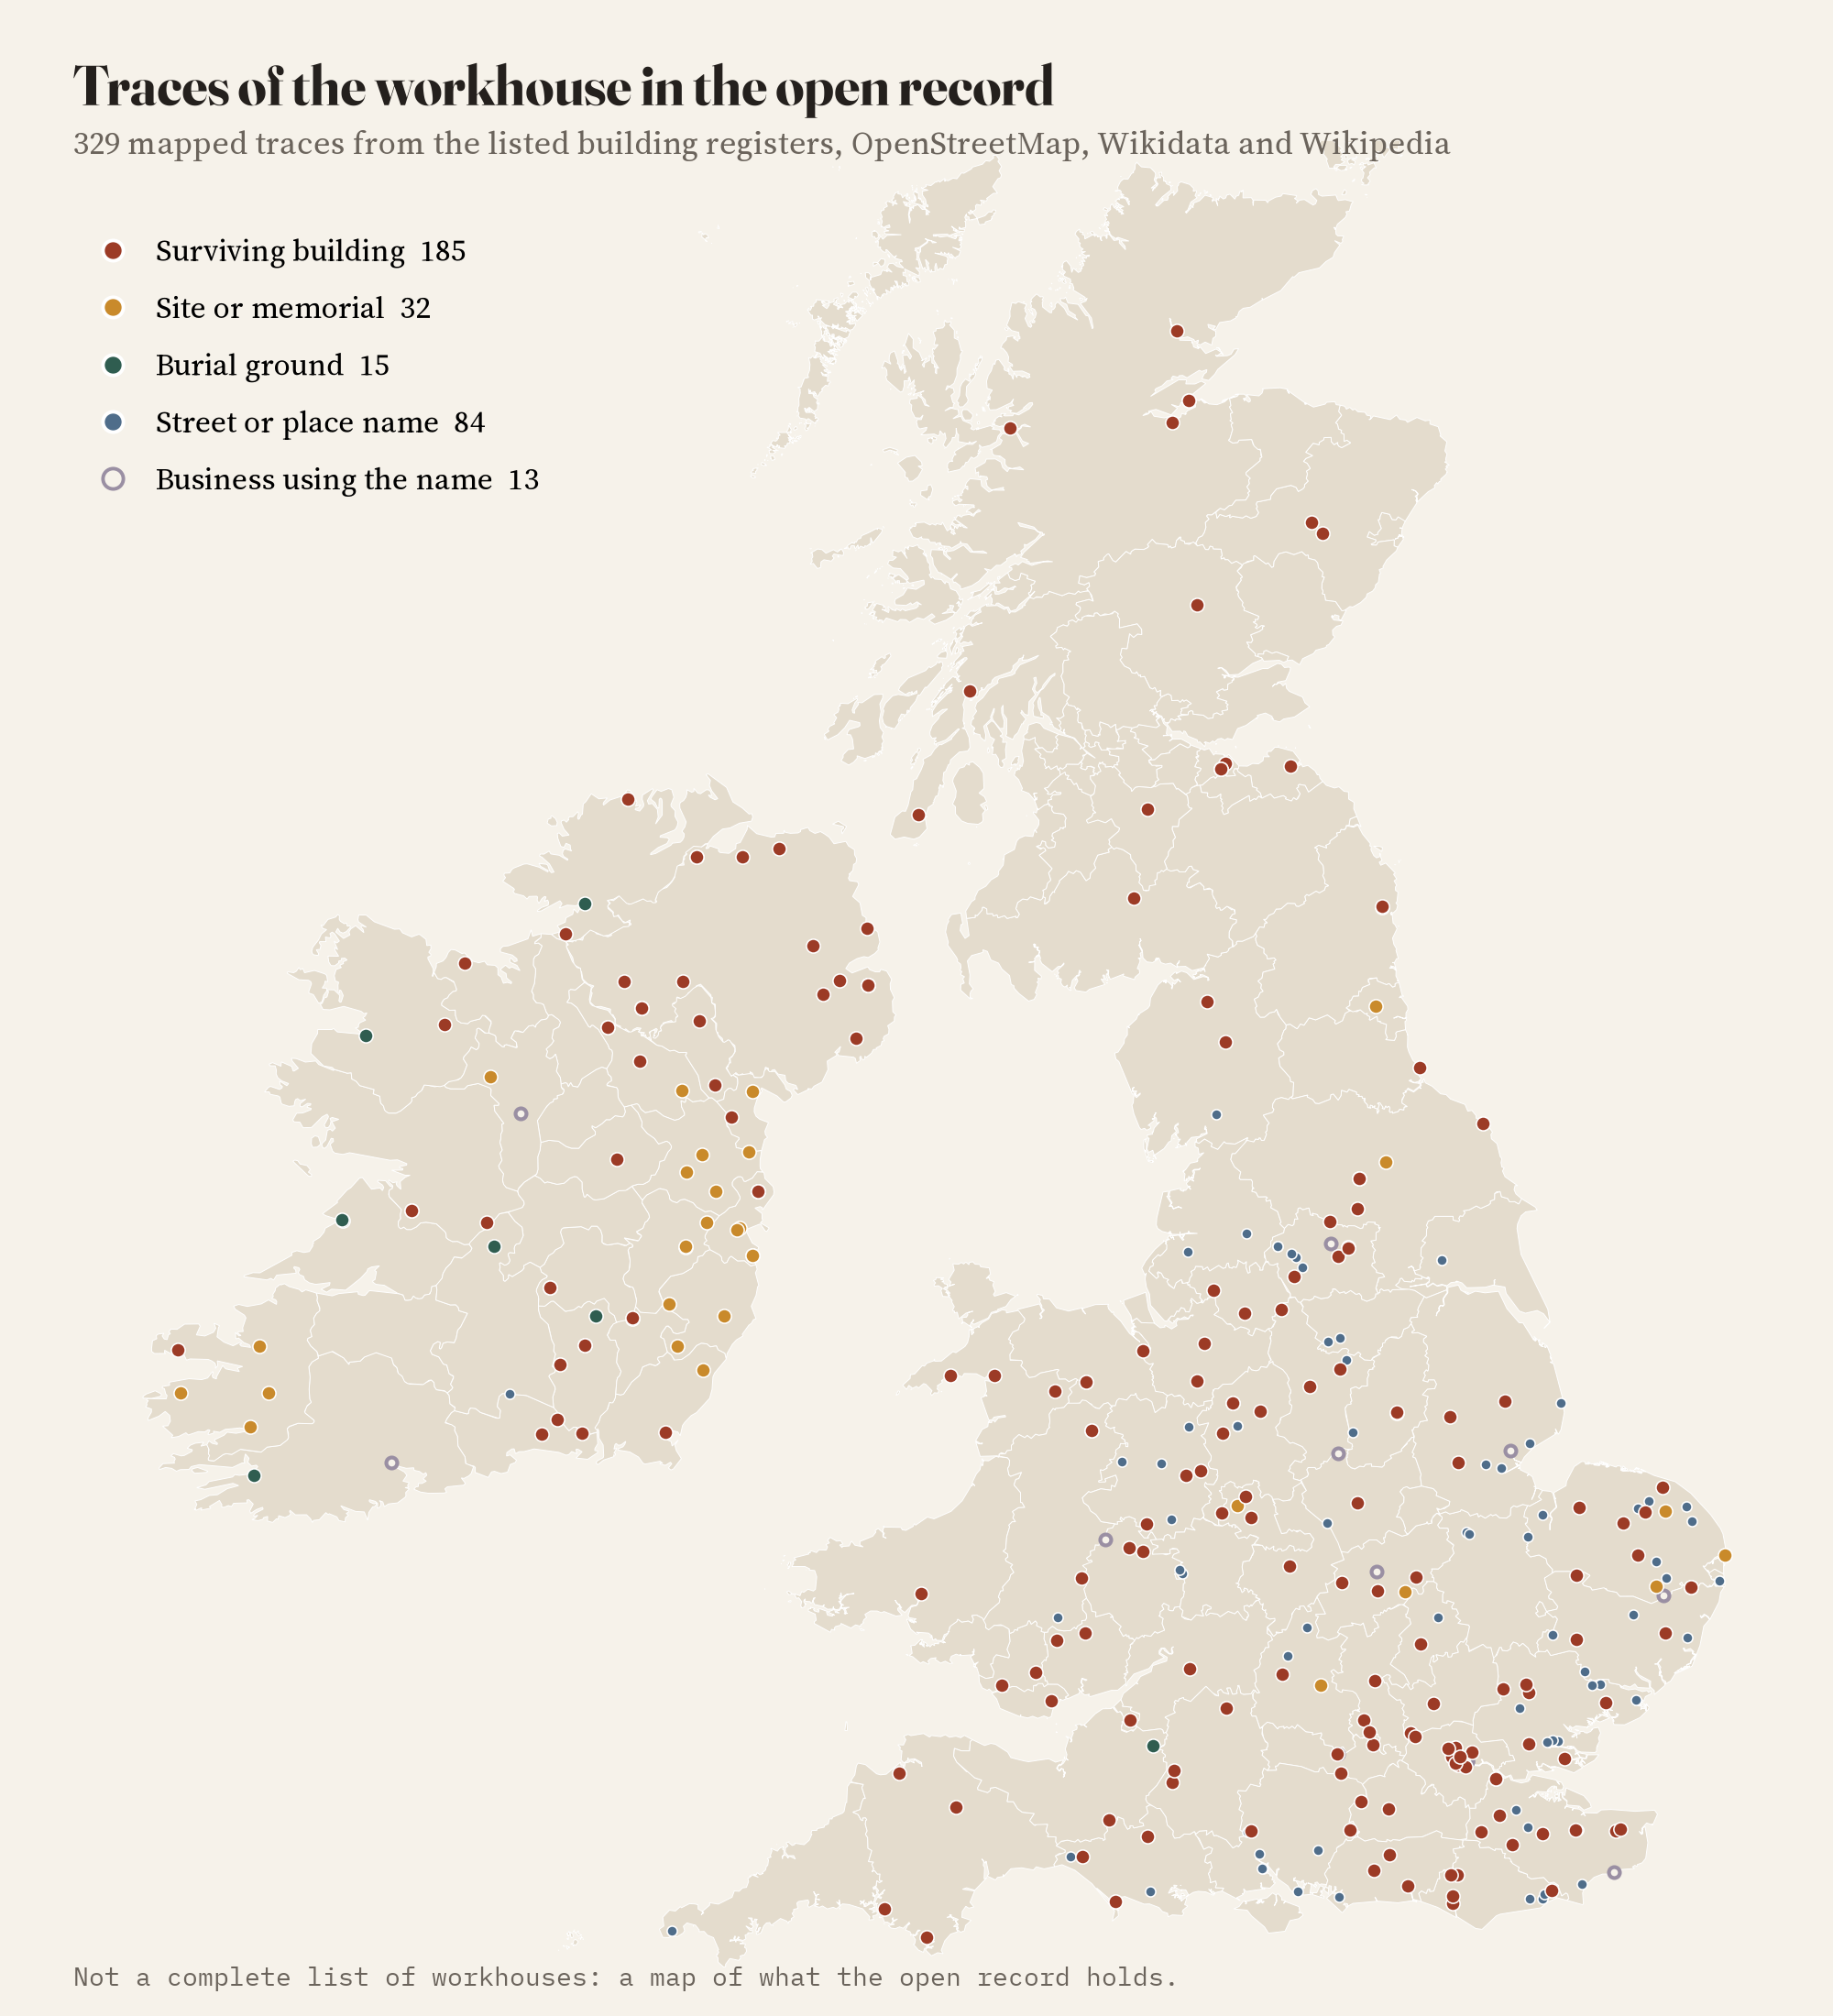
\includegraphics[width=.86\textwidth]{f_map.png}
\caption{Every mapped trace, by kind.}\label{fig:map}\end{figure}

\subsection{Sites and surviving buildings}
Grouping gives 205 sites: 168 with a surviving building, 28 known only as a site or memorial and 9 only as a burial ground (Figure~\ref{fig:sites}). 117 sites include a listed building. The 108 workhouse list entries are overwhelmingly of the lowest national grade: 96\% of those in England and Wales are Grade II, 2 are Grade II*, and the only Grade I is the poor house within Framlingham Castle, built in 1729. In England and Wales 14 entries call themselves a poor house, poorhouse or parish workhouse and 12 are simply `The Old Workhouse', against 29 that name a union, hundred or poor law institution: the listed record leans towards small eighteenth-century parish workhouses, which survive as houses and cottages, rather than union workhouses, which are often listed under a later hospital name that this search cannot find.

\begin{figure}[tbp]\centering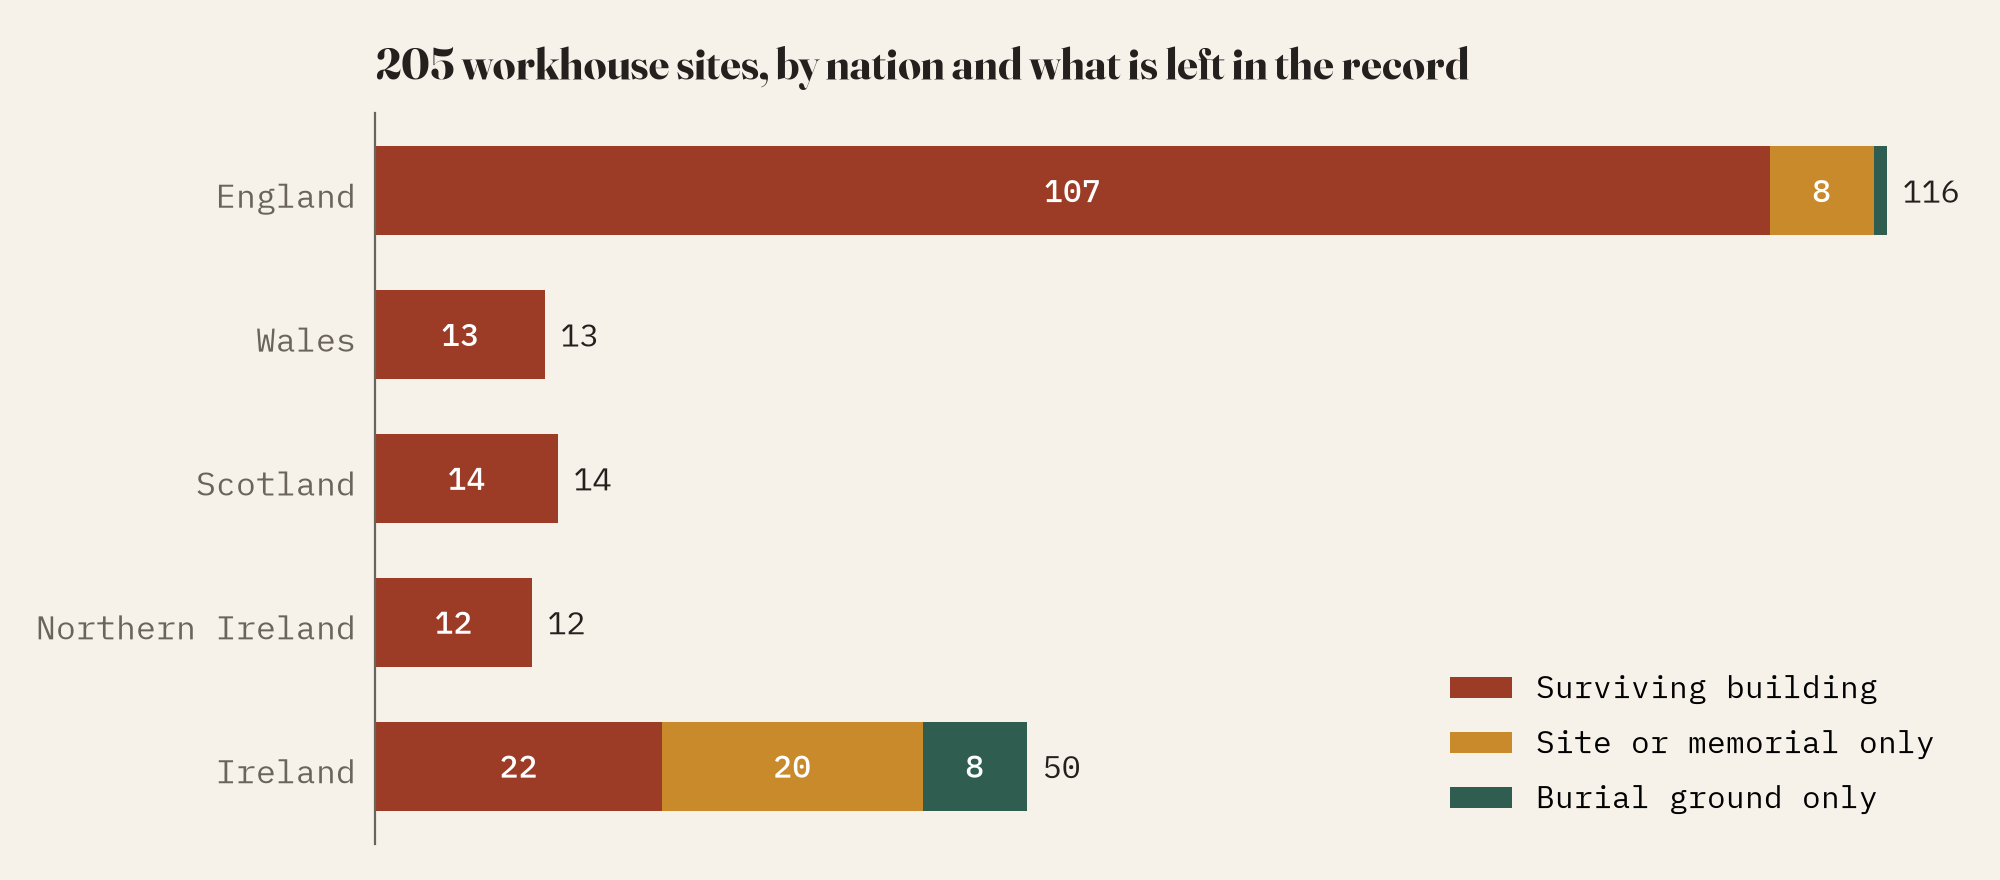
\includegraphics[width=.9\textwidth]{f_sites.png}
\caption{Workhouse sites by nation and what survives in the record.}\label{fig:sites}\end{figure}

\subsection{What surviving workhouses became}
The record states a later use for 80 of the 168 sites with a surviving building (48\%). Hospitals or health buildings (30, 38\%) and homes (29, 36\%) dominate, followed by museums or heritage sites (8), offices or community buildings (5), ruins (4), businesses (3) and a school (1) (Figure~\ref{fig:reuse}). The pattern follows the institutional history: infirmaries became municipal and then National Health Service hospitals, and as those hospitals closed many sites were converted to housing \citep{morrison}. The museums include the National Trust's workhouse at Southwell, Gressenhall in Norfolk, Llanfyllin in Powys, Ripon, the Cinema Museum in the former Lambeth workhouse, and the famine workhouses at Donaghmore and Dunfanaghy.

\begin{figure}[tbp]\centering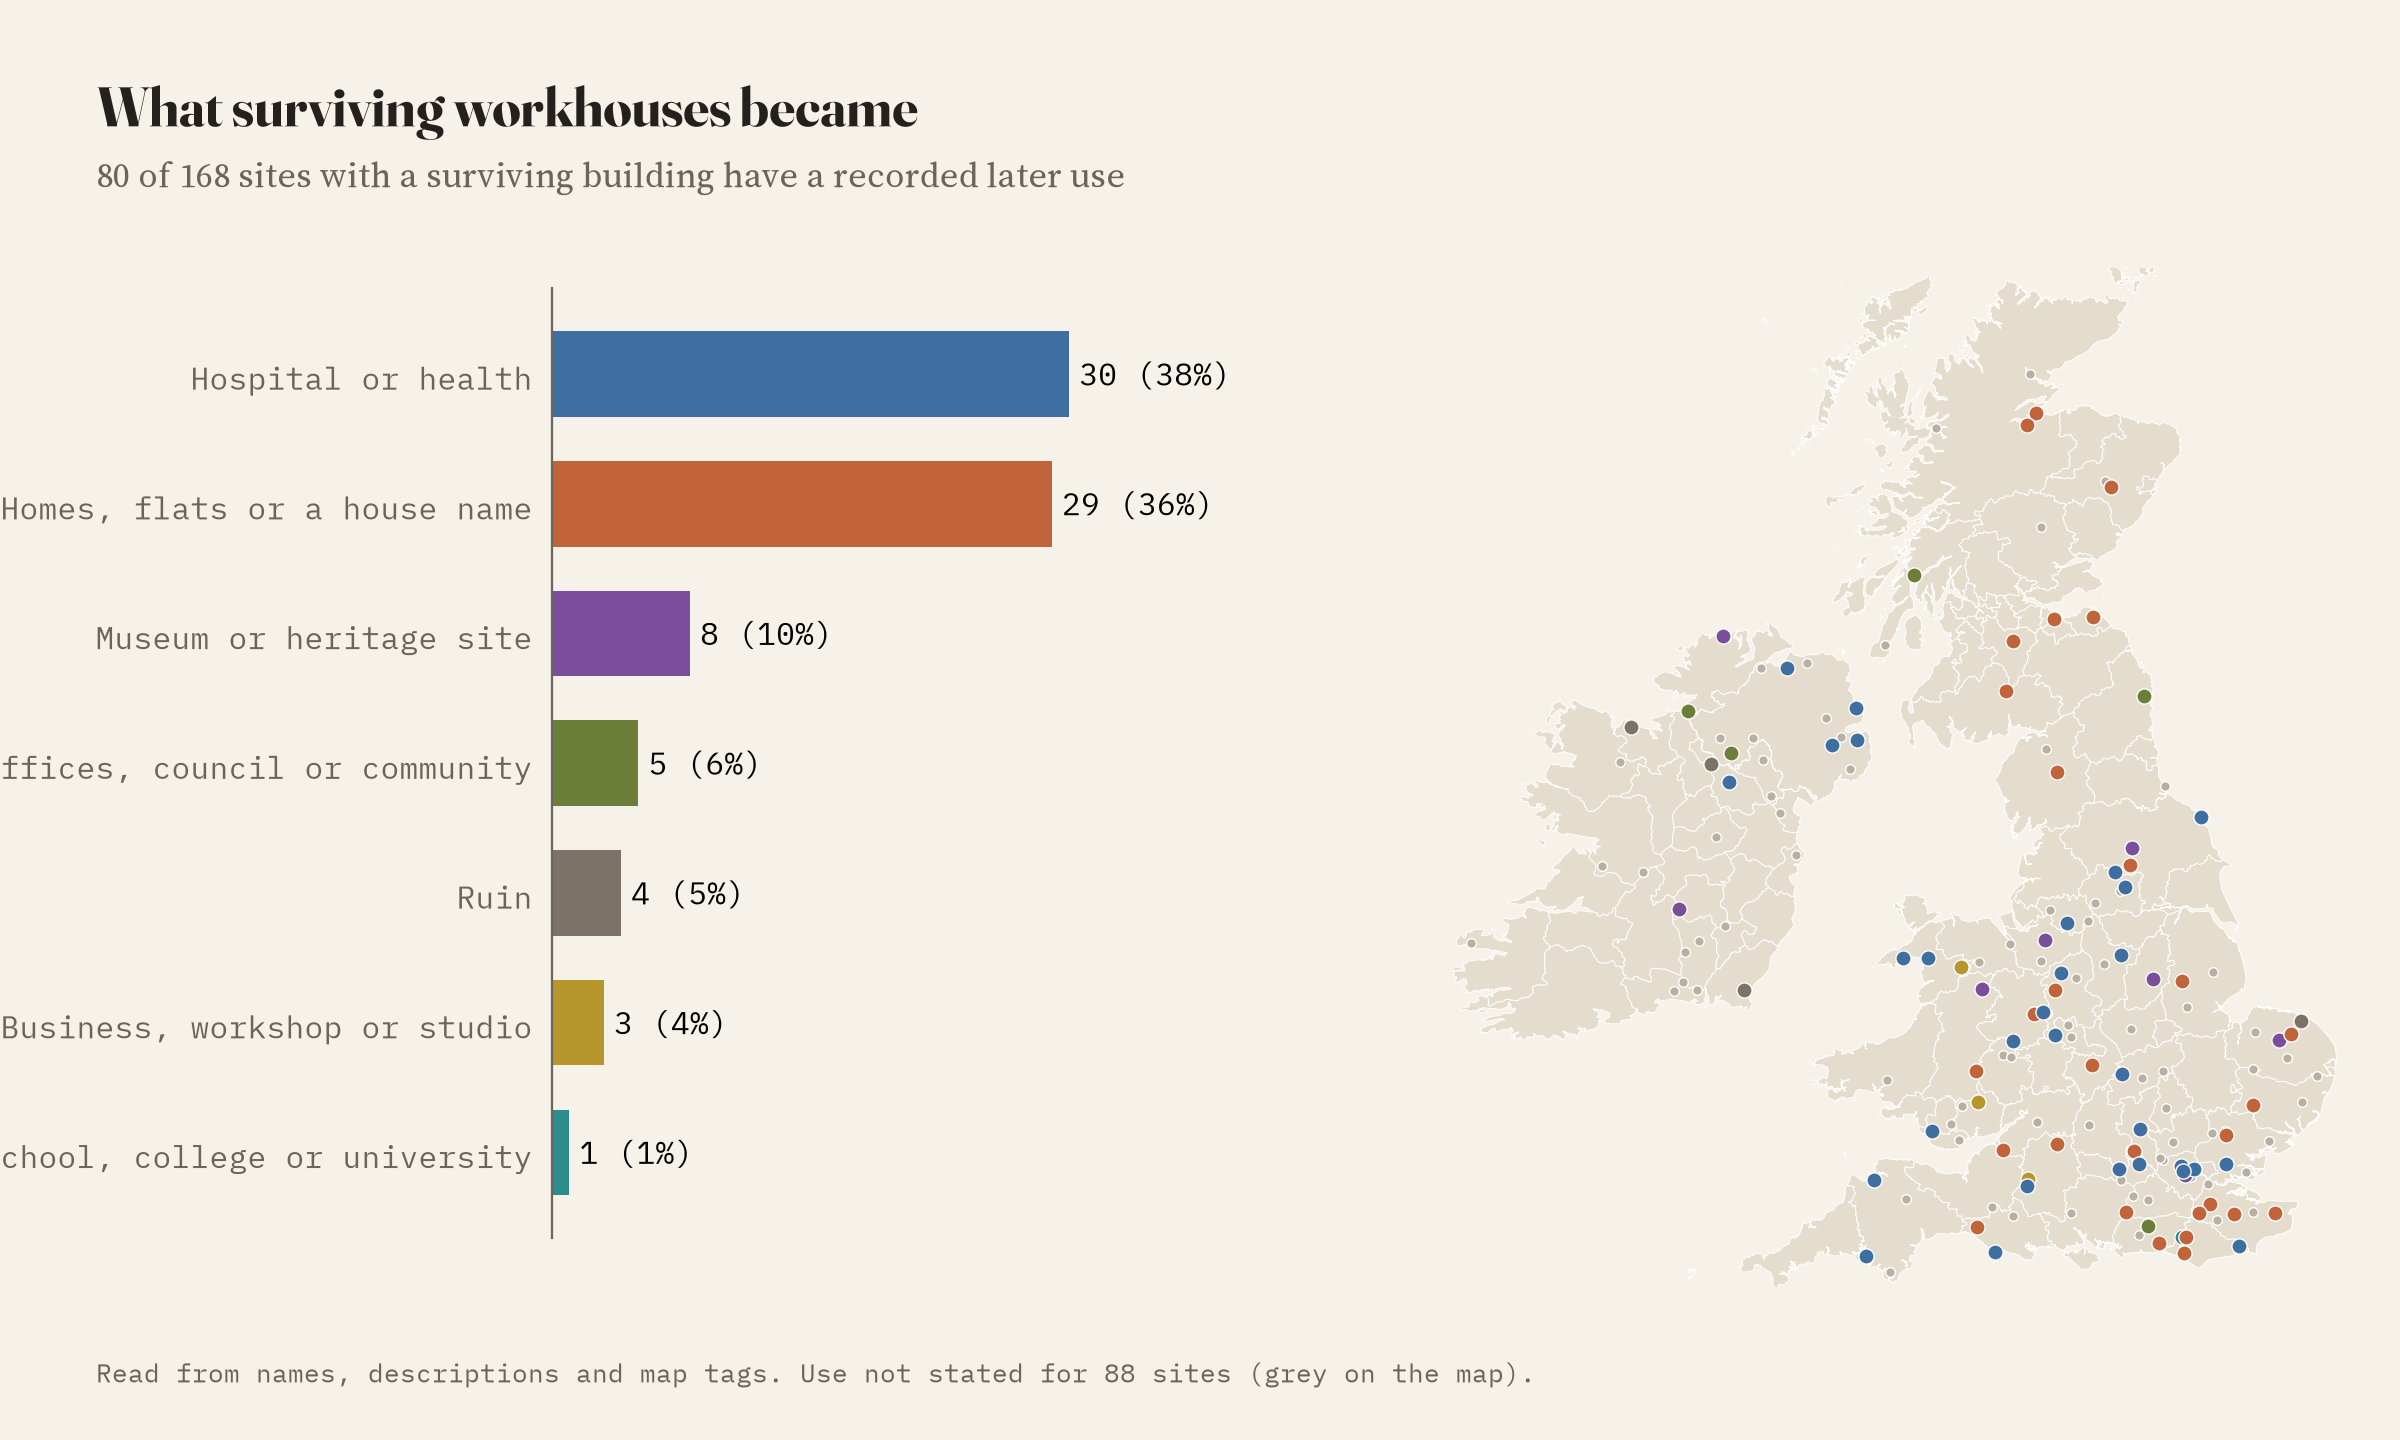
\includegraphics[width=\textwidth]{f_reuse.png}
\caption{Recorded later uses of surviving workhouse buildings, and the sites on the map (grey: use not stated).}\label{fig:reuse}\end{figure}

\subsection{Names}
84 streets, places and features carry the name (Figure~\ref{fig:names}): 32 lanes as well as roads, farms, woods, bridges, a brook, coppices, cycleways and hamlets such as Workhouse Green and Workhouse End. 71 use `workhouse' and 13 `poorhouse' or `poor house'. They are concentrated in England (92\%), especially the east and south: Essex and Norfolk have 8 each and Hampshire 7, and 34\% lie in the eastern counties from Lincolnshire to Essex. Most are rural and probably recall parish workhouses or their land. 13 businesses use the name, mostly gyms and cafés; 2 are at a workhouse site.

\begin{figure}[tbp]\centering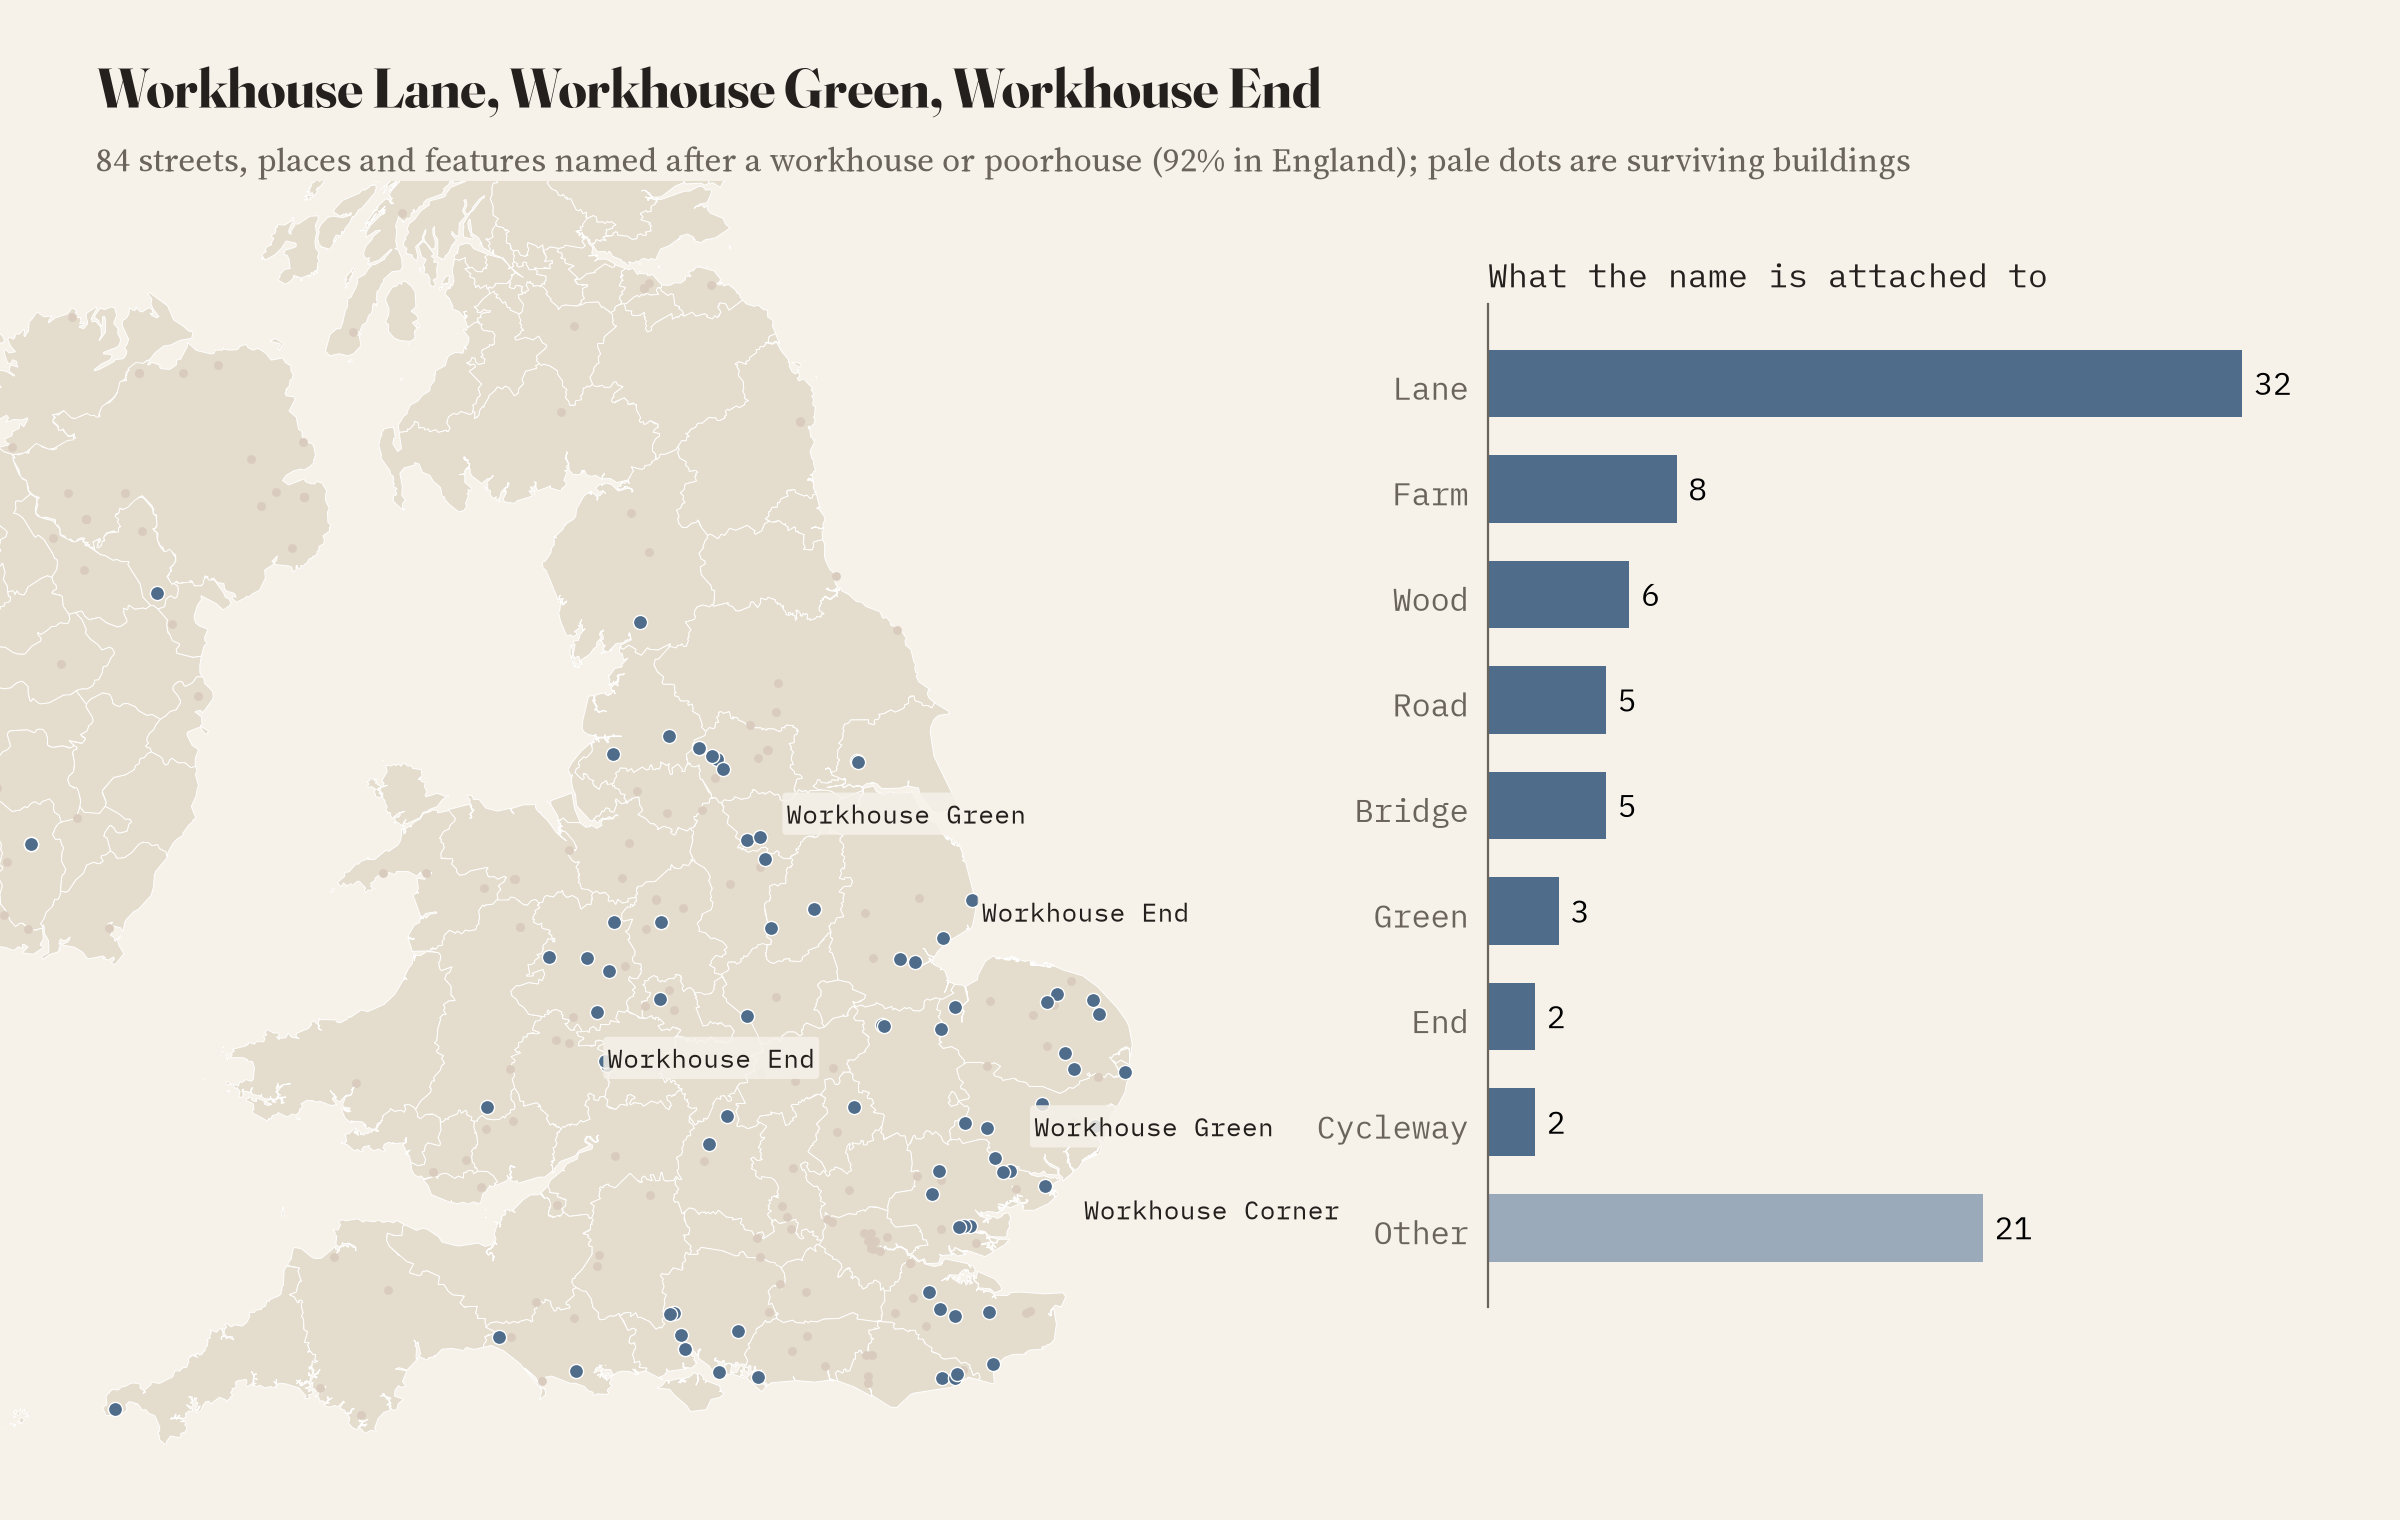
\includegraphics[width=\textwidth]{f_names.png}
\caption{Streets, places and features named after a workhouse or poorhouse.}\label{fig:names}\end{figure}

\subsection{Ireland}
On the island of Ireland there are 62 sites, 55\% with a surviving building in the record, against 94\% of 143 sites in Britain (Figure~\ref{fig:ireland}). In the Republic the figure is lower still: 22 of 50 sites, with 20 known only as sites and 8 only from burial grounds. Two things drive the difference. One is the sources: the Republic's architectural inventory is not included, and 21 Irish sites, in 9 counties mostly in Leinster and Kerry, come from OpenStreetMap features mapped as the `site of' a union workhouse. The other is history. Of the 15 mapped workhouse burial grounds, 14 are Irish (93\%), including workhouse graveyards, a cillín at Bantry and the cemeteries at Loughlinstown, Naas and Bawnboy; Britain's one is the Bath Union burial ground. A memorial at Kilkenny marks the remains of 970 famine victims found at the workhouse site in 2005, who died between August 1847 and March 1851. Two Irish traces carry the word famine in their name; none in Britain do.

\begin{figure}[tbp]\centering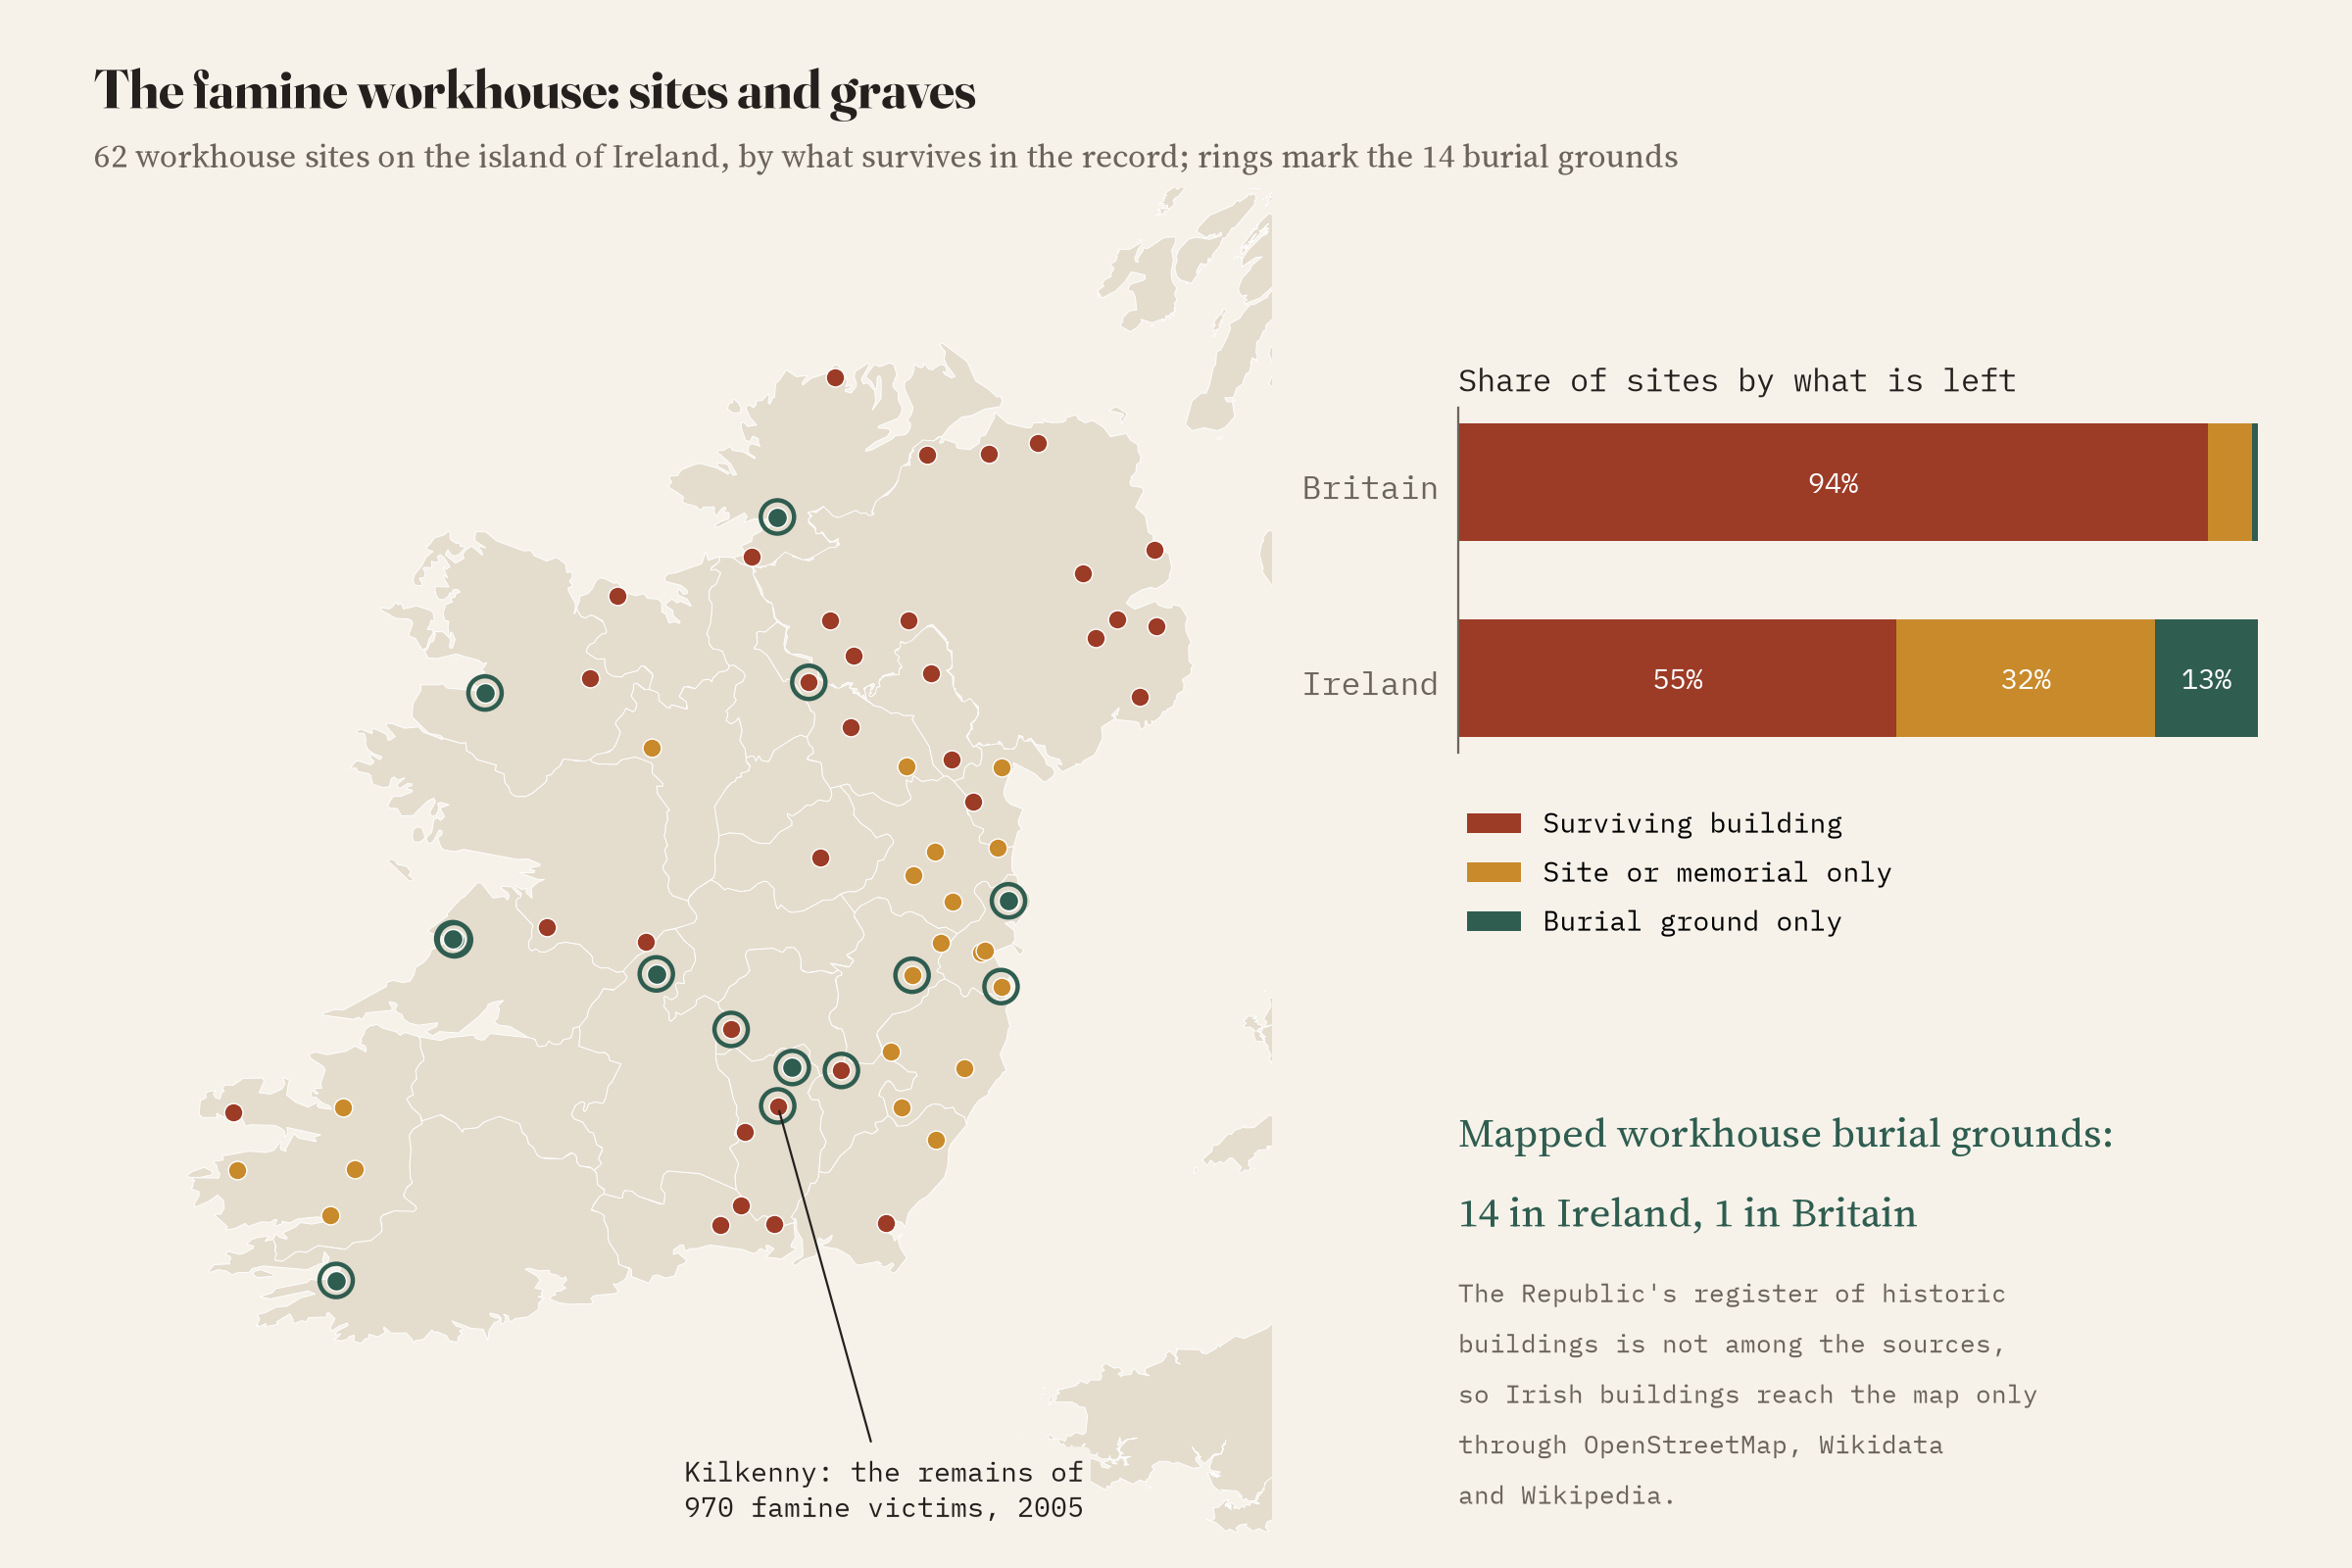
\includegraphics[width=\textwidth]{f_ireland.png}
\caption{Workhouse sites on the island of Ireland by status, with burial grounds ringed; share of sites by status in Britain and Ireland.}\label{fig:ireland}\end{figure}

\subsection{Completeness}
The sources overlap little: 168 of 205 sites (82\%) appear in only one source and 37 in two or more (Figure~\ref{fig:coverage}). Against the historical record the coverage is low. England and Wales had around 600 unions and many more parish workhouses, against 129 sites found; Ireland had 163 unions by the 1850s, against 62 sites (38\%); Scotland has 14.

\begin{figure}[tbp]\centering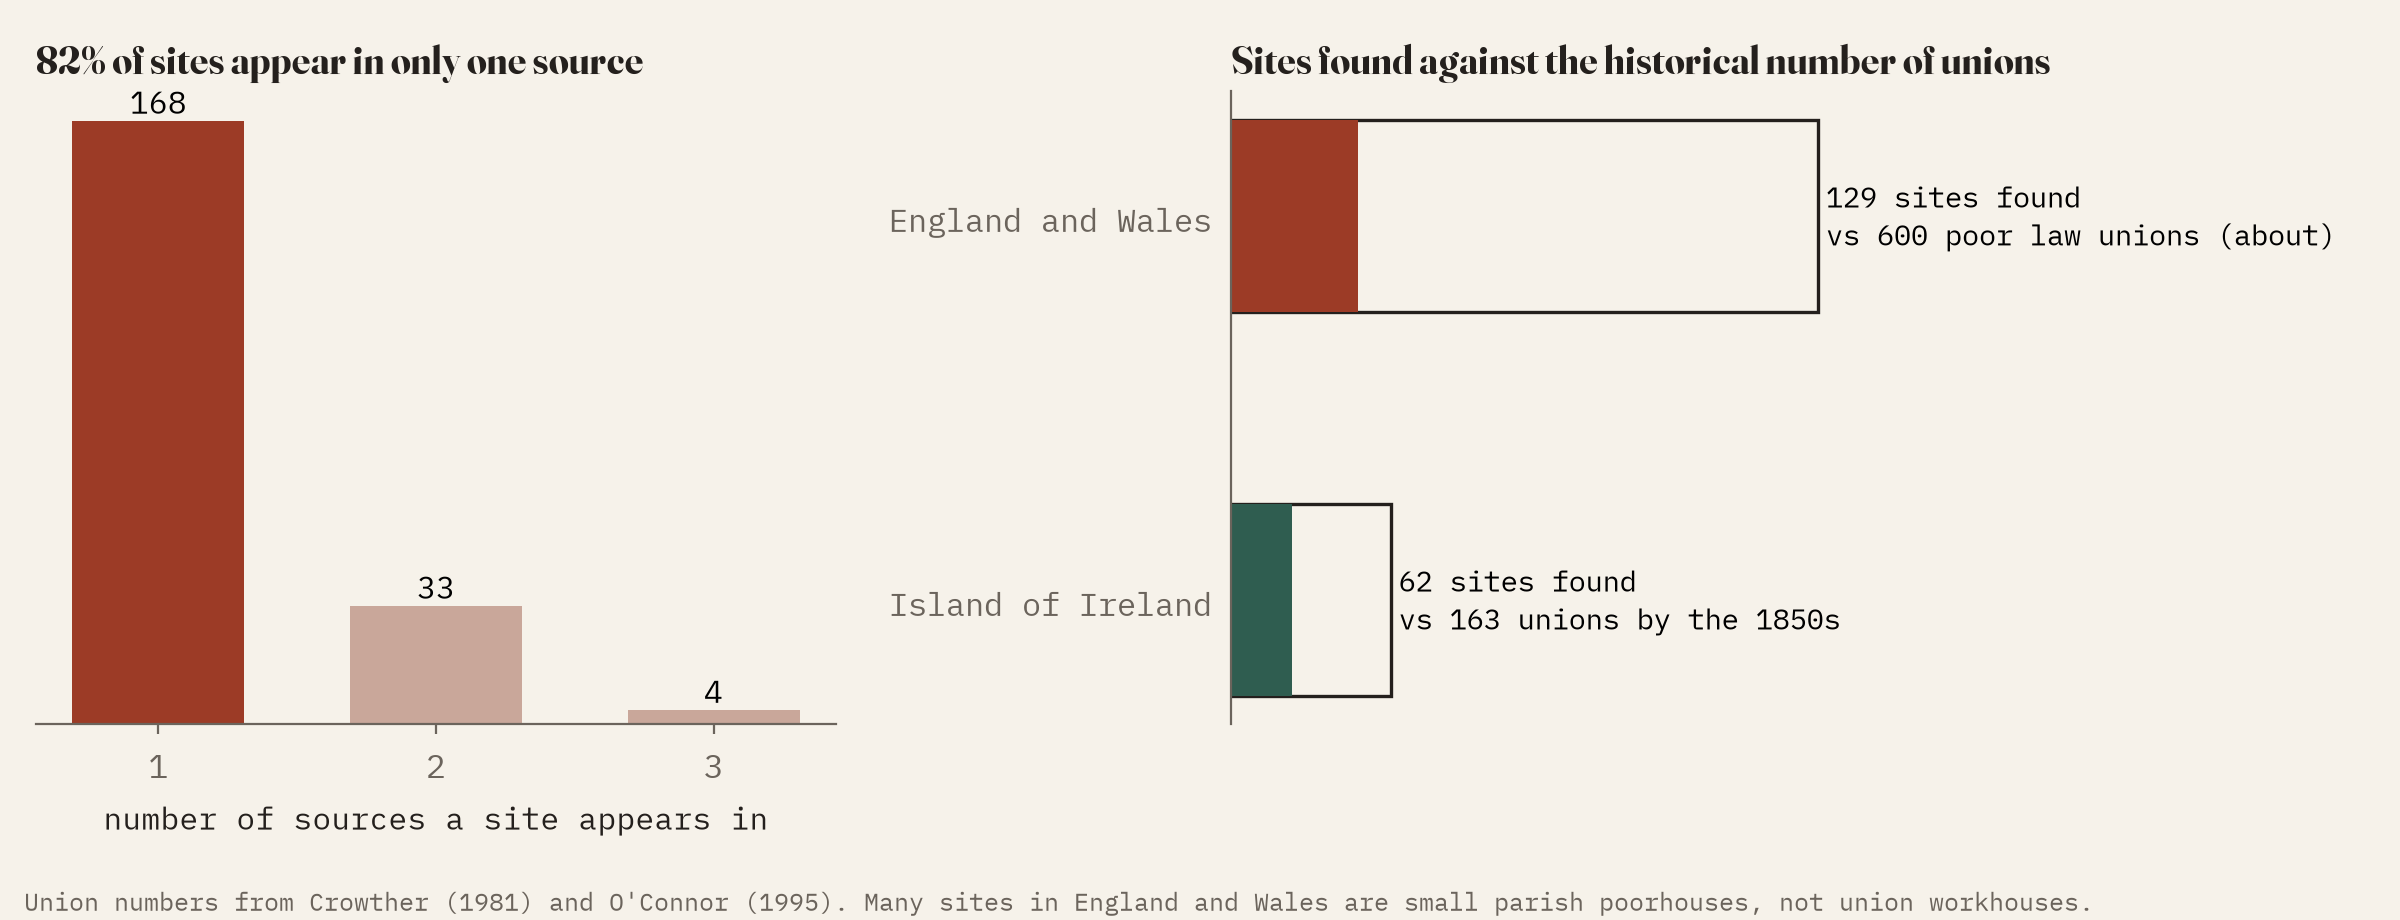
\includegraphics[width=\textwidth]{f_coverage.png}
\caption{Left: number of sources in which each site appears. Right: sites found against the historical number of poor law unions (from the literature).}\label{fig:coverage}\end{figure}

\section{Discussion}
Open data can say a good deal about the afterlife of the workhouse, even without a list of workhouses. Surviving buildings are mostly modest Grade II listings; the big union workhouses survive in the record chiefly as hospitals, and smaller ones as homes. The name survives where the building does not, in lanes and hamlets across eastern and southern England. And the Irish record is a record of loss: sites marked where buildings once stood, and burial grounds, the open-data shadow of the famine.

The study is equally a portrait of its sources. Each sees a different slice: the registers see listed fabric, but only when the entry's name mentions the workhouse; OpenStreetMap sees what volunteers have mapped, which explains the cluster of Irish `site of' features in Leinster and Kerry; Wikidata and Wikipedia see the famous and well documented. That 82\% of sites appear in a single source shows how much each source misses, and how much any one would miss alone.

\section{Limitations}
First, this is not a list of workhouses, and counts of traces must not be read as counts of workhouses or of their survival. Second, name searches miss workhouses listed or mapped under other names (most union workhouses that became hospitals) and include some false friends; I removed those I could identify, but some `Union House' entries remain probable rather than certain. Third, the Republic of Ireland's historic building inventory is not included, which lowers the Irish share of surviving buildings. Fourth, later uses are read from words and are known for fewer than half of the buildings; a house name is weak evidence of residential use. Fifth, grouping by distance can merge neighbouring institutions or split large sites. Finally, the historical comparison numbers come from the literature and are approximate.

\section{Conclusion}
What is left of the workhouse in the open record is a few hundred buildings, sites, names and graves: hospitals and flats in Britain, lanes and hamlets in eastern England, and in Ireland the burial grounds of the famine. The record is fragmentary and uneven, and the map should be read as a map of what is recorded. For the full history of any workhouse the place to go remains workhouses.org.uk and the literature cited here.

\section*{Data and code availability}
The interactive atlas is at \url{https://maps.tristanhotham.com/workhouses/}. Data and code are at \url{https://github.com/Tristan-Hotham/workhouses} and archived with this paper at \url{https://doi.org/10.5281/zenodo.23844517}. The traces table contains OpenStreetMap data and is released under the ODbL 1.0; other derived data and text under CC BY 4.0, and code under the MIT licence.

\section*{AI statement}
I wrote the text, with drafting and editing assistance from Claude (Anthropic), which also helped prepare the analysis code. I reviewed and checked all text and results.

\begin{thebibliography}{12}
\bibitem[Bast and Buchhold(2017)]{qlever} Bast, H. and Buchhold, B. (2017) QLever: a query engine for efficient SPARQL+text search. \emph{Proceedings of the 2017 ACM Conference on Information and Knowledge Management}, 647 to 656.
\bibitem[Crowther(1981)]{crowther} Crowther, M. A. (1981) \emph{The Workhouse System 1834-1929: The History of an English Social Institution}. London: Batsford.
\bibitem[Fowler(2007)]{fowler} Fowler, S. (2007) \emph{Workhouse: The People, the Places, the Life Behind Doors}. Kew: The National Archives.
\bibitem[Haklay and Weber(2008)]{osm} Haklay, M. and Weber, P. (2008) OpenStreetMap: user-generated street maps. \emph{IEEE Pervasive Computing}, 7(4), 12 to 18. Data: OpenStreetMap contributors, ODbL 1.0.
\bibitem[Higginbotham(2012)]{higginbotham} Higginbotham, P. (2012) \emph{The Workhouse Encyclopedia}. Stroud: The History Press. See also \url{https://www.workhouses.org.uk/}.
\bibitem[Hotham(2026)]{listed} Hotham, T. (2026) The Listed Kingdom: every listed building in the United Kingdom by grade, type, date of listing and date of building. Zenodo. \url{https://doi.org/10.5281/zenodo.23761429}
\bibitem[Kinealy(1994)]{kinealy} Kinealy, C. (1994) \emph{This Great Calamity: The Irish Famine 1845-52}. Dublin: Gill and Macmillan.
\bibitem[Morrison(1999)]{morrison} Morrison, K. (1999) \emph{The Workhouse: A Study of Poor-Law Buildings in England}. Swindon: English Heritage.
\bibitem[Natural Earth(2026)]{naturalearth} Natural Earth (2026) Admin 1 states and provinces and populated places (1:10m). Public domain.
\bibitem[O'Connor(1995)]{oconnor} O'Connor, J. (1995) \emph{The Workhouses of Ireland: The Fate of Ireland's Poor}. Dublin: Anvil Books.
\bibitem[Slack(1990)]{slack} Slack, P. (1990) \emph{The English Poor Law, 1531-1782}. Basingstoke: Macmillan.
\bibitem[Vrande\v{c}i\'{c} and Kr\"{o}tzsch(2014)]{wikidata} Vrande\v{c}i\'{c}, D. and Kr\"{o}tzsch, M. (2014) Wikidata: a free collaborative knowledgebase. \emph{Communications of the ACM}, 57(10), 78 to 85.
\end{thebibliography}
\end{document}
